\section{Activity Diagram}

\subsection{Printing service}
\begin{figure}[H]
\centering
  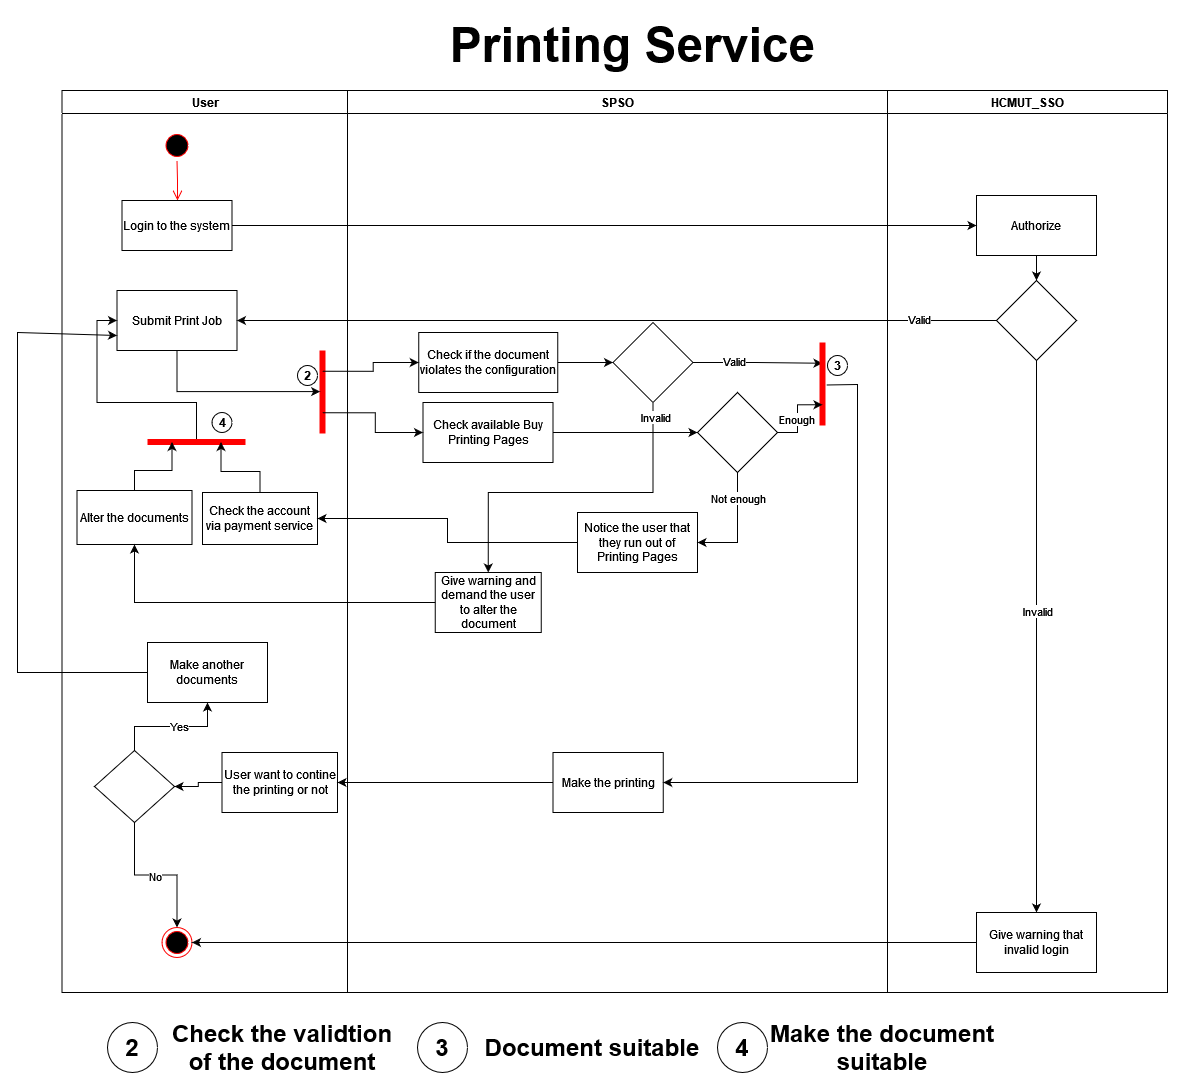
\includegraphics[max width=0.9\linewidth,origin = c]{chapters/4. system-modeling/activity/activity_printing.drawio.png}
  \caption{Activity diagram for Printing Service}%
\end{figure}

The printing service demonstrates the steps involved in producing printed documents. Initially, the user accesses the system by logging in through HCMUT\_SSO, which involves an authorization process. Once the user successfully logs into the website, they gain the ability to upload their documents for printing. At this point, the SPSO conducts two checks: it assesses the document's configuration and verifies the available remaining printing pages, akin to a "bank account" for printing. If any problems are identified during these checks, the user is notified and can make necessary adjustments before the printing process is finalized.

\subsection{View account status}

\begin{figure}[H]
\centering
  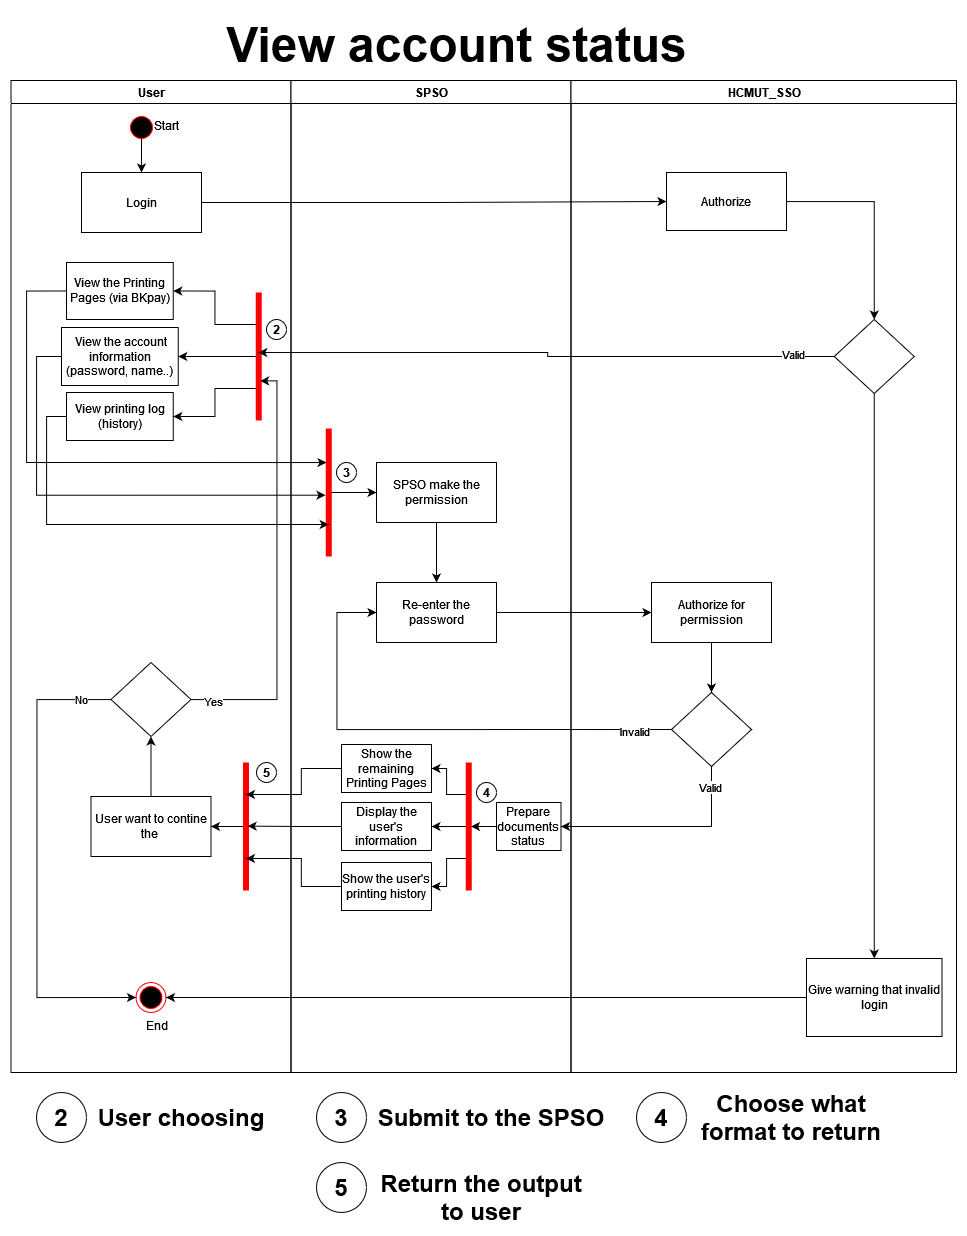
\includegraphics[max width=0.9\linewidth,origin = c]{chapters/4. system-modeling/activity/view account_acitivty.png}
  \caption{Activity diagram for View account status}%
\end{figure}

The "View account status" use-case enables users to access their personal account information, which includes their "bank account" balance, personal details, and printing history. Upon logging into the system via HCMUT\_SSO, users can request this information from the system. The SPSO (System for Printing Services and Operations) is responsible for generating the requested data and displaying it to the user. It's worth noting that users are required to re-enter their password before making the request to SPSO.

\subsection{Payment Service}

\begin{figure}[H]
\centering
  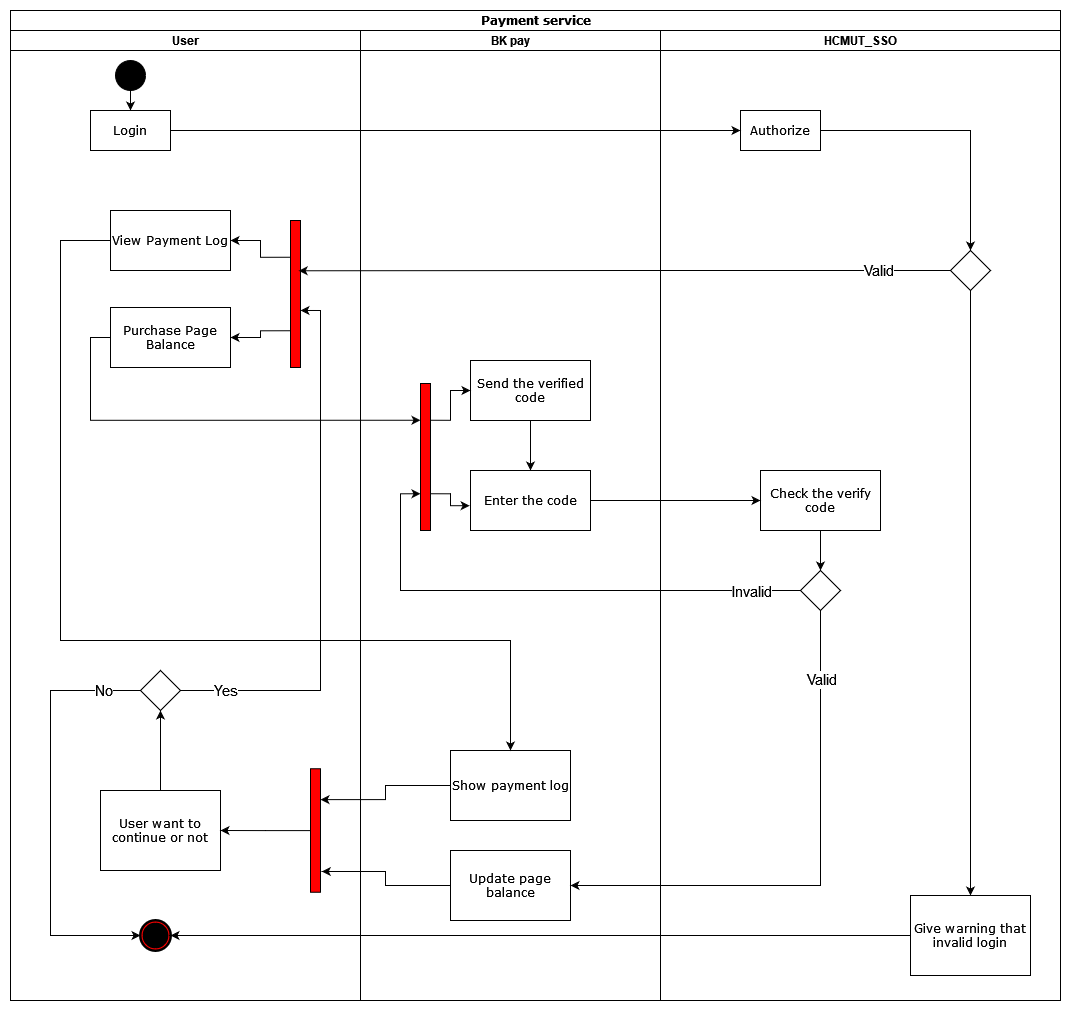
\includegraphics[max width=0.9\linewidth,origin = c]{chapters/4. system-modeling/activity/Activity_payment.png}
  \caption{Activity diagram for Payment Service}%
\end{figure}

The payment service allows students to purchase the balance and the school administrator can view the payment log. Initially, the user accesses the system by logging in through HCMUT\_SSO, which involves an authorization process. When logging into the system via HCMUT\_SSO, students can request the BKpay to purchase their balance. In order to purchase, students have to verify their transaction by receiving and entering the correct code. Students can request to resend the code if they haven’t received or they want to receive a new one to enter again. After finishing the transaction, the BKpay system will update the current balance for students.

\subsection{Report Service}

\begin{figure}[H]
\centering
  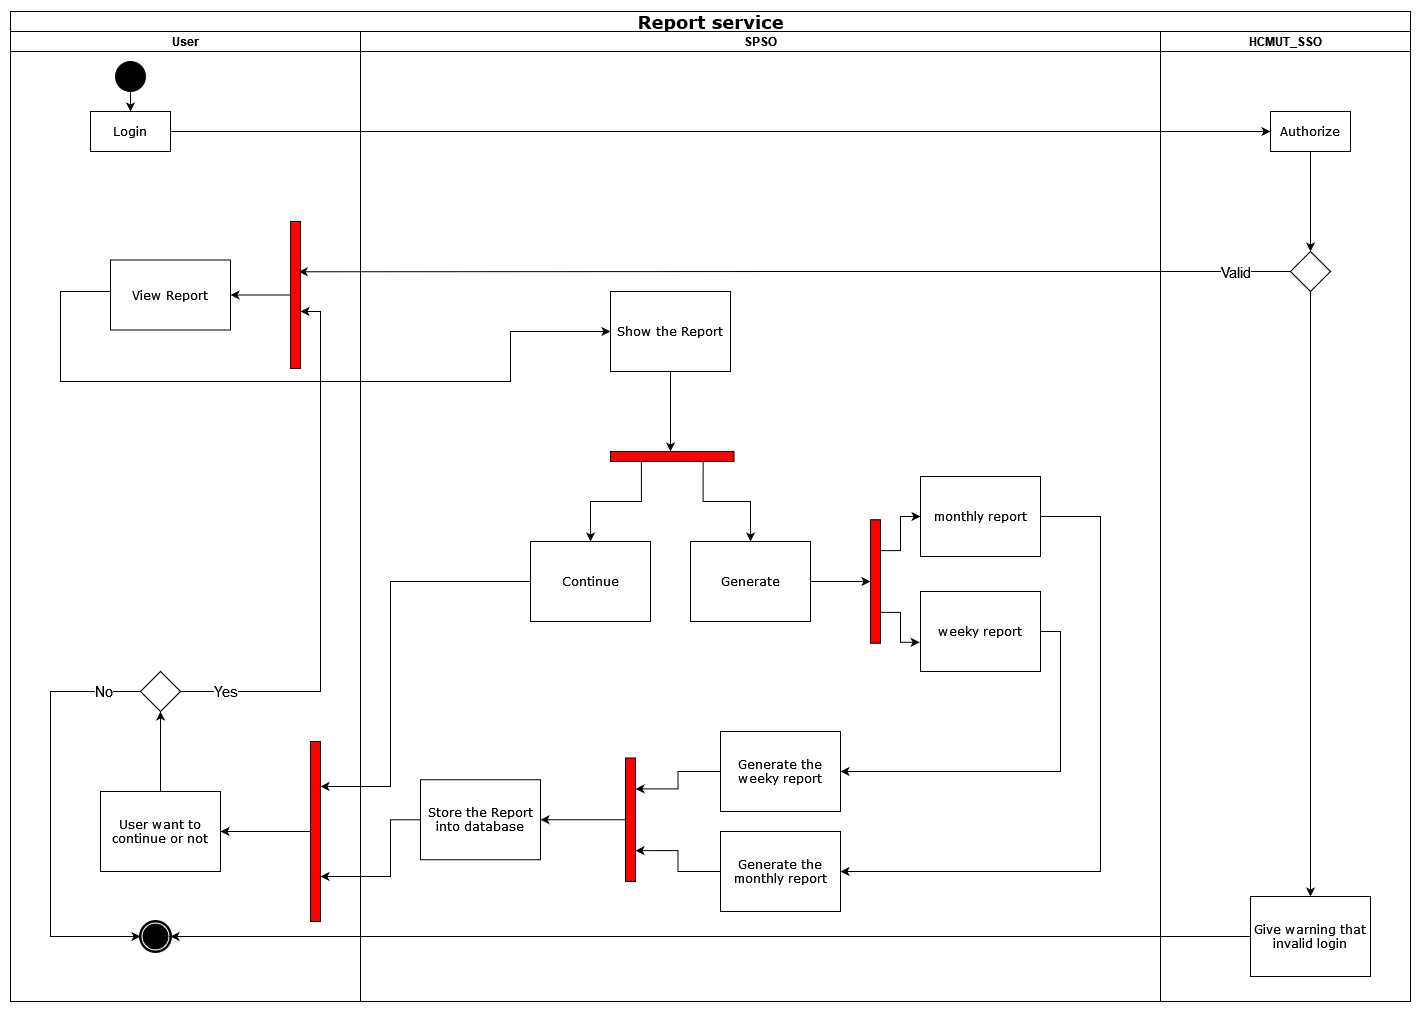
\includegraphics[max width=0.9\linewidth,origin = c]{chapters/4. system-modeling/activity/activity_report.png}
  \caption{Activity diagram for Report Service}%
\end{figure}

The report service enables users to view and generate the report. Initially, the user accesses the system by logging in through HCMUT\_SSO, which involves an authorization process. Upon logging into the system via HCMUT\_SSO, view the report from the Student Printing Service Officer. Users can request to generate the report on a weekly or monthly basis. After generate, the report will be stored into the database.












\section{Sequence Diagram}
\subsection{View Printer}                                                                        
\begin{figure}[H]
\centering
  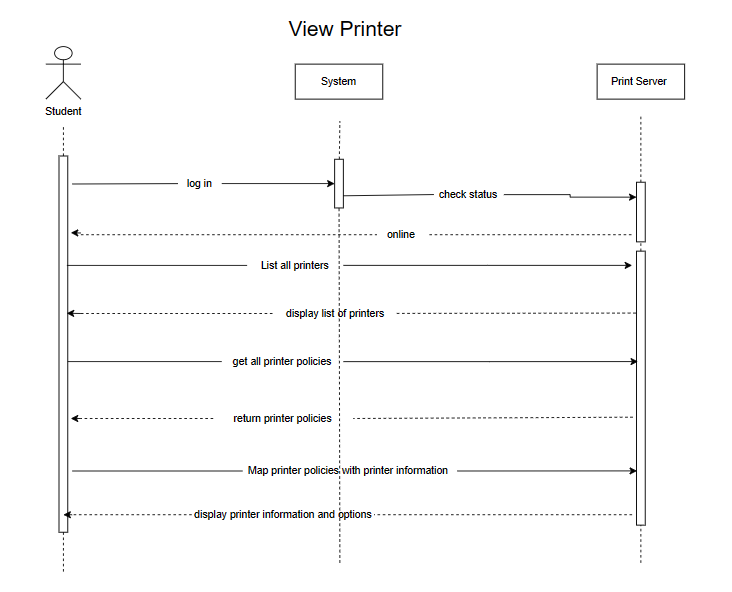
\includegraphics[max width=0.9\linewidth,origin = c]{chapters/4. system-modeling/picture/ViewPrinter.png}
  \caption{Sequence Diagram of View Printer}%
\end{figure}
Students login into the system, the system will check status in the print server and send server status (running) back to the students. The students will request to see all printers. The print server will display a list of all printers to the student. The students will request to see all printer policies. The print server will return all printer policies to the students. The server will map printer policies with printer information and display it back to students.
\subsection{View Printing Logs}
\begin{figure}[H]
\centering
  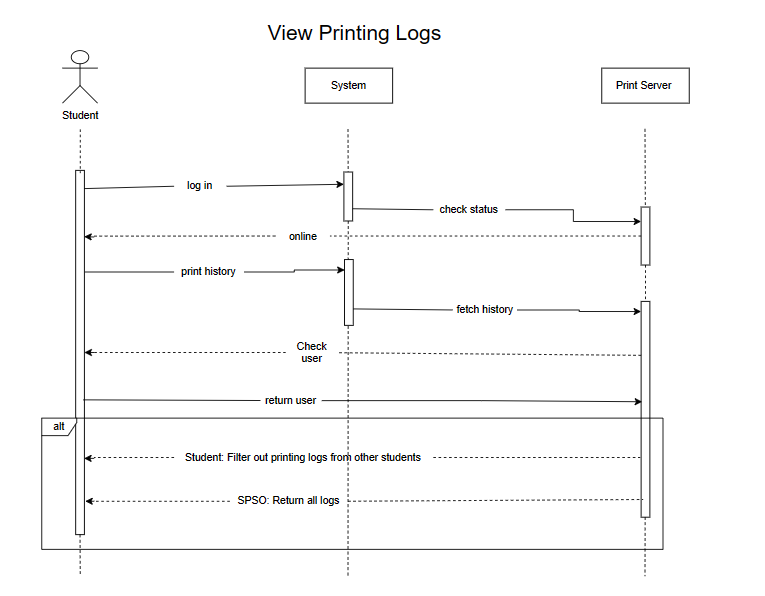
\includegraphics[max width=0.9\linewidth,origin = c]{chapters/4. system-modeling/picture/ViewPrintingLogs.png}
  \caption{Sequence Diagram of View Printing Logs}%
\end{figure}
Users login into the system, the system will check status in the print server and send server status (running) back to the students. The users send the request to print history to the system. The system will fetch the logs into the print server. The server will check the status of the user. User will return the status back to the server. If the user is a student, we will filter out printing logs from other students, if the user is Student Printing Service Officer, we will return all logs.

\subsection{Manage Printer Policies}
\begin{figure}[H]
\centering
  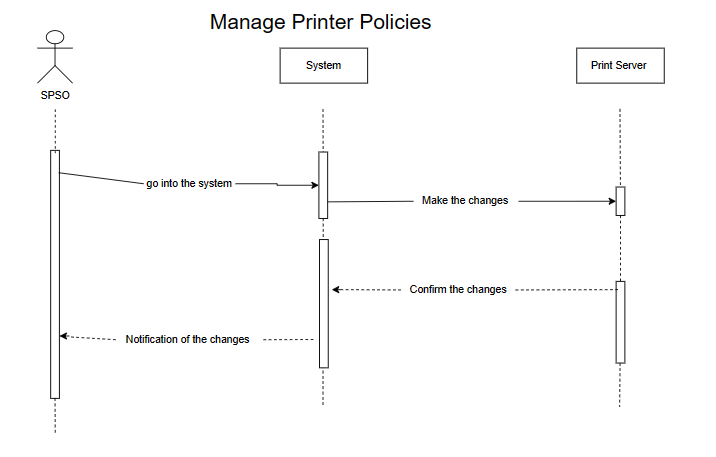
\includegraphics[max width=0.9\linewidth,origin = c]{chapters/4. system-modeling/picture/ManagePrinterPolicies.png}
  \caption{Sequence Diagram of Manage Printer Policies}%
\end{figure}
SPSO goes into the system, makes the changes in the print server. The server then will send the confirmation of the changes to the system. The system will notify the SPSO that the changes are applied.
\subsection{Log Out}
\begin{figure}[H]
\centering
  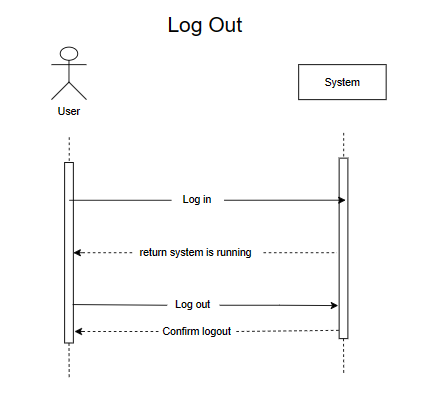
\includegraphics[max width=0.9\linewidth,origin = c]{chapters/4. system-modeling/picture/LogOut.png}
  \caption{Sequence Diagram of Log Out}%
\end{figure}
Users login into the system. The system will send server status (running) back to the users. The Users log out of the system. The system confirms the logging out.

\subsection{Submit Print Job}
\begin{figure}[H]
\centering
  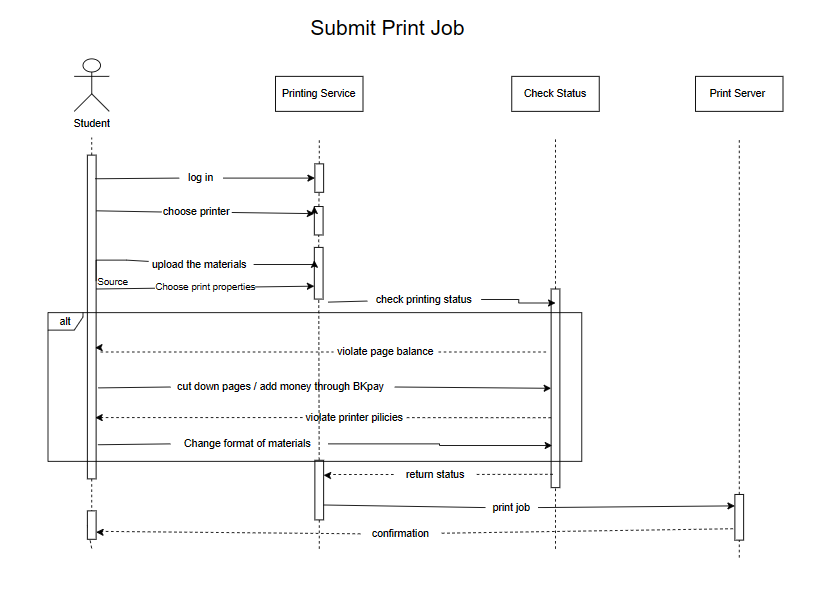
\includegraphics[max width=0.9\linewidth,origin = c]{chapters/4. system-modeling/picture/SubmitPrint.png}
  \caption{Sequence Diagram of the Submit Print Job}%
\end{figure}
Students login into the printing service, choose the printer and upload the materials. The printing service will check the status for these 2 exception flows. If it violates the page balance, students are required to cut down pages or add money through Bkpay2. If it violates the printer policies, students must change the format of the materials that meet the accepted configuration of the system. Then the status will be returned to the printing service. The submission of the print job will be sent from printing service to print server. The confirmation will be sent back to the user.

\section{Class Diagram}
\begin{figure}[H]
  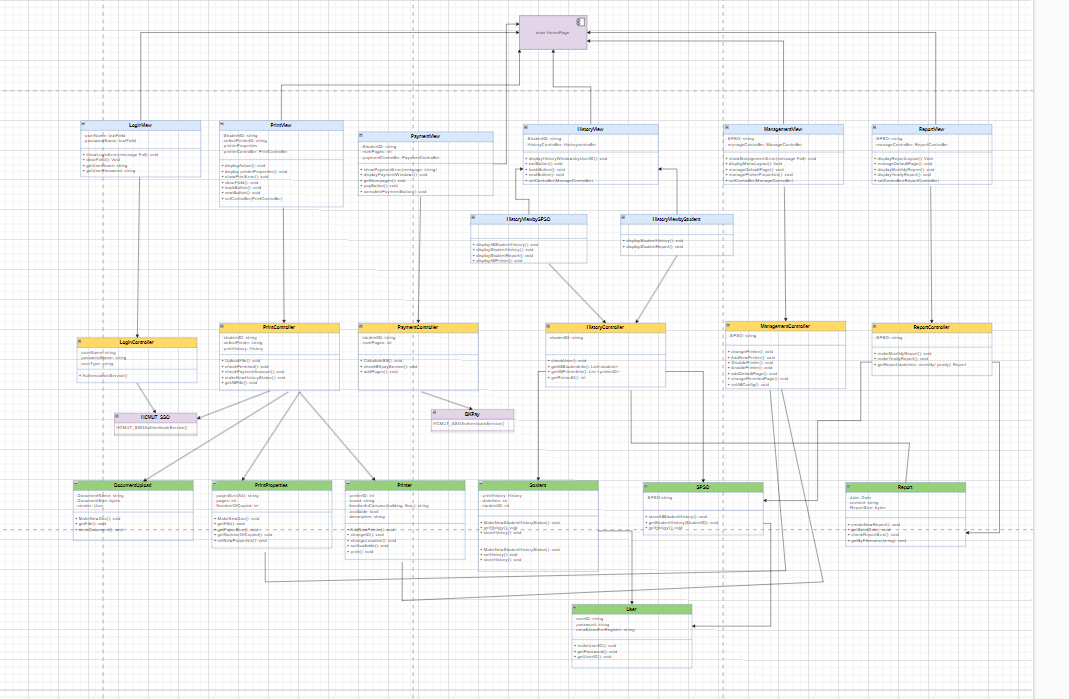
\includegraphics[max width=0.9\linewidth,origin = c]{chapters/4. system-modeling/picture/class.PNG}
  \caption{Class Diagram}%
\end{figure}

The class diagram presents a structured view of a system with classes that cover various aspects of a school management system, including printing services, payment, user history, and report generation. Notably, there is a \textbf{LoginView} class that likely handles user authentication, which is connected to a \textbf{LoginController}. There's an inheritance hierarchy where SPSO classes inherit from Student and User classes respectively, indicating different types of users. The \textbf{HistoryController} class is connected to two different views, suggesting that it handles the logic for displaying historical data for both staff and students. \textbf{ReportController} manages report generation, while \textbf{PaymentController} seems to deal with financial transactions. The Printer class has a composition relationship with \textbf{PrintProperties} and \textbf{DocumentUpload}, indicating that printing functionality is central to this system. Overall, the diagram suggests a comprehensive system designed to manage various administrative tasks in an educational setting.\\

Overall, The diagram illustrates a multi-faceted educational institution management system, integrating various functionalities such as authentication, printing, payment processing, and report management. It emphasizes modularity and object-oriented design, with clear divisions between user interfaces, control logic, and data models. There are specific pathways for user interaction flows and data processing, indicating a system capable of handling complex, interrelated tasks while maintaining a separation of concerns for easier maintenance and scalability.\\

For further references see \href{https://drive.google.com/file/d/15Wbk8DiISW-IV2xAhueTpo-qr4kJO3H4/view?usp=sharing}{Class Diagram on drawio}